%%%%%%%%%%%%%%%%%%%%%%%%%%%%%%%%%%%%%%%%%
% Thesis 
% LaTeX Template
% Version 1.3 (21/12/12)
%
% This template has been downloaded from:
% http://www.latextemplates.com
%
% Original authors:
% Steven Gunn s
% http://users.ecs.soton.ac.uk/srg/softwaretools/document/templates/
% and
% Sunil Patel
% http://www.sunilpatel.co.uk/thesis-template/
%
% License:
% CC BY-NC-SA 3.0 (http://creativecommons.org/licenses/by-nc-sa/3.0/)
%
% Note:
% Make sure to edit document variables in the Thesis.cls file
%
%%%%%%%%%%%%%%%%%%%%%%%%%%%%%%%%%%%%%%%%%

%----------------------------------------------------------------------------------------
%	PACKAGES AND OTHER DOCUMENT CONFIGURATIONS
%----------------------------------------------------------------------------------------

\documentclass[11pt, a4paper, oneside]{timetabling-notes} % Paper size, default font size and one-sided paper

%extras
\usepackage{verbatim}
\usepackage{epigraph}
\usepackage{float}
\usepackage{tikz}
\usepackage{gantt}
\usepackage{multirow}
\usepackage{graphics}
\usepackage{tabu}
\usepackage{listings}
\usepackage{xcolor}
\usepackage{amssymb}% http://ctan.org/pkg/amssymb
\usepackage{pifont}% http://ctan.org/pkg/pifont
\newcommand{\cmark}{\ding{51}}%
\newcommand{\xmark}{\ding{55}}%
\usepackage{slashbox}
\usepackage{lscape}
\usepackage{pdflscape}
\usepackage{amsmath}
\usepackage{algorithm}
\usepackage{caption}
\usepackage[noend]{algpseudocode}


\usepackage{xcolor,colortbl}
\definecolor{green}{rgb}{0,1,0}
\definecolor{red}{rgb}{1,0,0}

\newcommand{\ccheck}{\cellcolor{green}\cmark}  %{0.9}
\newcommand{\xcheck}{\cellcolor{red}\xmark}

\colorlet{punct}{red!60!black}
\definecolor{background}{HTML}{EEEEEE}
\definecolor{delim}{RGB}{20,105,176}
\colorlet{numb}{magenta!60!black}

\taburulecolor{black}



\graphicspath{{./Pictures/}} % Specifies the directory where pictures are stored

\usepackage[square, numbers, comma, sort&compress]{natbib} % Use the natbib reference package - read up on this to edit the reference style; if you want text (e.g. Smith et al., 2012) for the in-text references (instead of numbers), remove 'numbers' 
\hypersetup{urlcolor=blue, colorlinks=false} % Colors hyperlinks in blue - change to black if annoying
\title{\ttitle} % Defines the thesis title - don't touch this


\begin{document}

\frontmatter % Use roman page numbering style (i, ii, iii, iv...) for the pre-content pages

\setstretch{1.3} % Line spacing of 1.3

% Define the page headers using the FancyHdr package and set up for one-sided printing
\fancyhead{} % Clears all page headers and footers
\rhead{\thepage} % Sets the right side header to show the page number
\lhead{} % Clears the left side page header

\pagestyle{fancy} % Finally, use the "fancy" page style to implement the FancyHdr headers

\newcommand{\HRule}{\rule{\linewidth}{0.5mm}} % New command to make the lines in the title page

% PDF meta-data
\hypersetup{pdftitle={\ttitle}}
\hypersetup{pdfsubject=\subjectname}
\hypersetup{pdfauthor=\authornames}
\hypersetup{pdfkeywords=\keywordnames}

%----------------------------------------------------------------------------------------
%	TITLE PAGE
%----------------------------------------------------------------------------------------

\begin{titlepage}
\begin{center}

\textsc{\LARGE \univname}\\[1.5cm] % University name
\textsc{\Large Draft}\\[0.5cm] % Thesis type
\textsc{}\\[0.5cm] % Thesis type

\HRule \\[0.4cm] % Horizontal line
{\huge \bfseries \ttitle}\\[0.4cm] % Thesis title
\HRule \\[1.5cm] % Horizontal line
 

\large
\center\emph{Author:}\\
\authornames % Author name - remove the \href bracket to remove the link

\begin{minipage}{0.4\textwidth}
\begin{flushright} \large
\emph{} \\
\supname % Supervisor name - remove the \href bracket to remove the link  
\end{flushright}
\end{minipage}\\[3cm]
 
 
{\large \today}\\[2cm] % Date

\vfill
\end{center}

\end{titlepage}

%----------------------------------------------------------------------------------------
%	QUOTATION PAGE
%----------------------------------------------------------------------------------------


\pagestyle{empty} % No headers or footers for the following pages

\begin{comment}
\null\vfill % Add some space to move the quote down the page a bit

\textit{``Insert fancy quote here."}

\begin{flushright}
Me
\end{flushright}

\vfill\vfill\vfill\vfill\vfill\vfill\null % Add some space at the bottom to position the quote just right

\clearpage % Start a new page
\end{comment}
%----------------------------------------------------------------------------------------
%	ABSTRACT PAGE
%----------------------------------------------------------------------------------------

\addtotoc{Abstract} % Add the "Abstract" page entry to the Contents

\abstract{\addtocontents{toc}{\vspace{1em}} % Add a gap in the Contents, for aesthetics


Timetabling is a difficult combinatorial optimization problem mainly because there are a lot of constraints to be satisfied and a huge search space to be explored. Since the past fifty years, this problem has been studied and a lot of different techniques, with varied success appeared to tackle the problem. In this work an architecture of an engine capable of generating timetables is described. It also shown an example of a possible approach that could be followed. This example is based on a two-stage algorithm where a feasible timetable is first achieved through a simple constructive heuristic and is followed by an iterated local search algorithm with neighbourhood structures able to generate similar solutions and solutions with major differences in order to search different regions of the search space.   


\textbf{Keywords:} \keywordnames timetabling, combinatorial optimization problem, computational complexity, constraint satisfaction, iterated local search, neighbourhood operators

\clearpage % Start a new page

%----------------------------------------------------------------------------------------
%	ACKNOWLEDGEMENTS
%----------------------------------------------------------------------------------------

\begin{comment}
\setstretch{1.3} % Reset the line-spacing to 1.3 for body text (if it has changed)

\acknowledgements{\addtocontents{toc}{\vspace{1em}} % Add a gap in the Contents, for aesthetics

}
\clearpage % Start a new page
\end{comment}

%----------------------------------------------------------------------------------------
%	LIST OF CONTENTS/FIGURES/TABLES PAGES
%----------------------------------------------------------------------------------------

\pagestyle{fancy} % The page style headers have been "empty" all this time, now use the "fancy" headers as defined before to bring them back

\lhead{\emph{Contents}} % Set the left side page header to "Contents"
\tableofcontents % Write out the Table of Contents

\lhead{\emph{List of Figures}} % Set the left side page header to "List of Figures"
\listoffigures % Write out the List of Figures

\lhead{\emph{List of Tables}} % Set the left side page header to "List of Tables"
\listoftables % Write out the List of Tables

\lhead{\emph{List of Algorithms}}
\listofalgorithms



%----------------------------------------------------------------------------------------
%	ABBREVIATIONS
%----------------------------------------------------------------------------------------

\clearpage % Start a new page

\setstretch{1.5} % Set the line spacing to 1.5, this makes the following tables easier to read

\lhead{\emph{Abbreviations}} % Set the left side page header to "Abbreviations"

\listofsymbols{ll} % Include a list of Abbreviations (a table of two columns)
{
\textbf{HTML} & \textbf{H}yper\textbf{T}ext \textbf{M}arkup \textbf{L}anguage \\
\textbf{RIA} & \textbf{R}ich \textbf{I}nternet \textbf{A}pplication \\
\textbf{ODBC} & \textbf{O}pen  \textbf{D}atabase  \textbf{C}onnectivity \\
\textbf{NP} & \textbf{N}ondeterministic \textbf{P}olynomial \textbf{T}ime \\
\textbf{CLP} & \textbf{C}onstraint \textbf{L}ogic \textbf{P}rogramming \\
\textbf{SQL} & \textbf{S}tructured \textbf{Q}uery \textbf{L}anguage \\
\textbf{MVC} & \textbf{M}odel \textbf{V}iew \textbf{C}ontroller \\
\textbf{PATAT} & \textbf{P}ractice \textbf{A}nd \textbf{T}heory of \textbf{A}utomated \textbf{T}imetabling \\
\textbf{WATT} & \textbf{W}orking group on \textbf{A}utomated \textbf{T}ime\textbf{T}abling\\
\textbf{POJO} &  \textbf{P}lain \textbf{O}ld \textbf{J}ava \textbf{O}bject



}

\begin{comment}
%----------------------------------------------------------------------------------------
%	PHYSICAL CONSTANTS/OTHER DEFINITIONS
%----------------------------------------------------------------------------------------

\clearpage % Start a new page

\lhead{\emph{Physical Constants}} % Set the left side page header to "Physical Constants"

\listofconstants{lrcl} % Include a list of Physical Constants (a four column table)
{
Speed of Light & $c$ & $=$ & $2.997\ 924\ 58\times10^{8}\ \mbox{ms}^{-\mbox{s}}$ (exact)\\
% Constant Name & Symbol & = & Constant Value (with units) \\
}

%----------------------------------------------------------------------------------------
%	SYMBOLS
%----------------------------------------------------------------------------------------

\clearpage % Start a new page

\lhead{\emph{Symbols}} % Set the left side page header to "Symbols"

\listofnomenclature{lll} % Include a list of Symbols (a three column table)
{
$a$ & distance & m \\
$P$ & power & W (Js$^{-1}$) \\
% Symbol & Name & Unit \\

& & \\ % Gap to separate the Roman symbols from the Greek

$\omega$ & angular frequency & rads$^{-1}$ \\
% Symbol & Name & Unit \\
}
\end{comment}

%----------------------------------------------------------------------------------------
%	DEDICATION
%----------------------------------------------------------------------------------------
%
%\setstretch{1.3} % Return the line spacing back to 1.3
%
%\pagestyle{empty} % Page style needs to be empty for this page
%
%\dedicatory{To Who? \ldots} % Dedication text
%
%\addtocontents{toc}{\vspace{2em}} % Add a gap in the Contents, for aesthetics

%----------------------------------------------------------------------------------------
%	THESIS CONTENT - CHAPTERS
%----------------------------------------------------------------------------------------

\mainmatter % Begin numeric (1,2,3...) page numbering

\pagestyle{fancy} % Return the page headers back to the "fancy" style

% Include the chapters of the thesis as separate files from the Chapters folder
% Uncomment the lines as you write the chapters

% Chapter 1

\chapter{Introduction} % Main chapter title
%\epigraph{If you can't explain it simply, you don't understand it well enough.}{Albert Einstein}

\label{intro} % For referencing the chapter elsewhere, use \ref{Chapter1} 

\lhead{Chapter 1. \emph{Introduction}} % This is for the header on each page - perhaps a shortened title

This chapter provides a quick overview of the theme, its importance and the motivation for this work.
%----------------------------------------------------------------------------------------

\section{Motivation}

Timetabling is an activity that is constantly present in our daily lives and contributes to a better organized society. The process of automated timetabling can be applied to many areas such as transportation, education (school, class or examination timetabling), work (employee timetabling), health services, sports, etc. In other words, this process is attached to any activity that needs to schedule a set of events, usually specifying meetings where people should meet at a given place and time. This work focus on university class timetabling, i.e., the scheduling of a set of classes, teachers, rooms and students at a fixed number of time slots.\\ 
Due to the relevance of timetabling in our society, it is very important not only to achieve valid methods of constructing timetables but also methods that produce timetables of good quality. Usually, the amount of existing resources (rooms, time slots, people, etc.) is limited. Therefore, this is a very challenging problem since the resulting timetables must respect a given set of desirable objectives like space usage and a large variety of user preferences. \\
The manual process of constructing a timetable is a very tedious and laborious activity, since it involves many person-days of work or even weeks to produce a satisfactory timetable, requiring a great investment of time and concentration. Besides, there is normally a single opportunity to make it right, with the possibility of making minor modifications at the end and thus, the option of trying alternative scenarios is reduced greatly. In most of the cases, the resulting solutions have poor quality in terms of resource allocation or faculty satisfaction.\\ The satisfaction of a timetable is usually given by the number of requirements it meets. These requirements usually fall into one of the following categories \citep{syllabus}:
\begin{itemize}
	\item Educational - Usually, it is not desirable for students to have large contiguous blocks of classes from the same or related subjects (e.g.: Mathematical Analysis right after Analytical Geometry or Japanese right after a German class.) 
	\item Work conditions of the staff - For example, the teacher and student loads should be distributed through the day and through the week, i.e., there should be a number of free periods in order to distribute the load evenly.
	\item Political reasons - Certain teachers may be working on part-time and therefore are only available in certain times, or may have other commitments like research projects.
\end{itemize} 

Timetabling is 10\% theory and 90\% politics \citep{waterloo}. Usually, the objectives that a timetable must or should meet are very diverse, specific to the institution where they are being applied and sometimes some of them conflict with each other. Therefore, some  trade-offs have always to be considered.\\
The timetabling problem is a very well-known combinatorial optimization problem in Computer Science. This means that the objective is to find the best assignment (according to the imposed constraints and user preferences) of values to variables, which in our case means choosing a time slot and a room to each event that needs to be scheduled. The complexity of the problem is related to the number of events that are needed to be scheduled and the objectives that must satisfy. In fact, this problem belongs to the class of NP-complete problems \citep{Garey_Johnson_1979}, which means that the problem is so difficult that currently all known algorithms need an exponential amount of time to discover the best solution, i.e., there is not yet a known algorithm that can solve the problem in a polynomial time. Given the nature of the problem, approximation algorithms are usually preferred to exact algorithms. Besides, the number of constraints in this problem varies from one institution to another. \\
One of the first works about this problem dates from the sixties by Gotlieb \citep{gotlieb1963}, in which he formulated a class-teacher problem. Since then, this has been a very active area and there are international competitions and special interest groups around the subject.

% Chapter 2
\hyphenation{student/teacher}

\chapter{Problem Definition} % Main chapter title
%\epigraph{A fancy quote.}{Me}

\label{current_process} % For referencing the chapter elsewhere, use \ref{Chapter2} 

\lhead{Chapter 2. \emph{Problem Definition}} % This is for the header on each page - perhaps a shortened title

This chapter explains some basic concepts commonly found in the literature. A comprehensive explanation of example constraints and their relative importance is also shown.  
%----------------------------------------------------------------------------------------

\section{Fundamental Concepts}

In order to better understand this work, it is important to define some concepts that may have different meanings in other works and in the literature. 

The following list of concepts is oriented to the Portuguese scenario \citep{bullet_paper} \citep{recent_dev_patat}.  

\begin{itemize}
	\item \textbf{Constraint} - A constraint is a specified rule that must or should be respected. If the constraint is specified as hard, then it must be followed. Soft constraint should be respected as much as possible.  
	\item \textbf{Conflict} - A conflict represents an undesirable situation where two events conflict somehow with each other (e.g., teachers in common at the same time slot) and must not happen.
	\item \textbf{Feasible Timetable} - A timetable is considered feasible when all events are scheduled and no hard constraint is violated.  
	\item \textbf{Course} - An Educational Institution may offer various courses. Each course has a set of curricular plans, usually one for each year of the duration of the course.
	\item \textbf{Curricular Plan} - A curricular plan is a set of subjects or disciplines to be taken by students wishing to obtain a given degree.
	\item \textbf{Subject} - A subject is a discipline taught one or more times a week, under different possible \textbf{typologies} (e.g., theoretical, practical). It is usually taught in a specific part of the year (e.g., annual, half a year, quarterly). Also, the same subject may be taught repeatedly for the different groups of students and is usually called a \textbf{turn} or \textbf{class}.  
	\item \textbf{Class} - A class represents a set of students having the same subject at the same time. This class may then be broken down in a couple of lectures (events) and this set of students remain together throughout the week. It is important to note that the schedules are defined at this level, i.e, this particular class will have a set of lectures scheduled along the week.
	\item \textbf{Group} - A group is a set of students who follow the same curricular plan and share the same timetable.
	\item \textbf{Event} - An event is the basic unit to be scheduled. It represents a lecture that is lectured by a teacher to a group of students, at a given time, with a given duration and occurs in a given classroom. Each event occurs in a set of weeks, representing the duration of the subject and is subject to a set of constraints that should or must be respected. 
	\item \textbf{Time slot} - A time slot is the basic time unit and it is associated to the assigned events. An event may have a duration of several time slots.
\end{itemize}

Figure \ref{fig:portuguese_curr_plan} illustrates some of these concepts.
 	   
\begin{figure}[htbp]
	\centering
		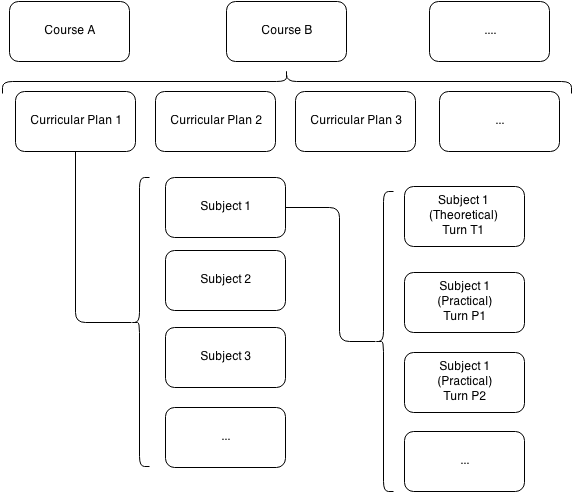
\includegraphics[scale=0.55]{./Figures/curricular_structure.png}
		\rule{35em}{0.5pt}
	\caption[The university curricular structure in Portugal]{The university curricular structure in Portugal}
	\label{fig:portuguese_curr_plan}
\end{figure}

There are many variations of the timetabling problem. When students, teachers and classes are involved, we are usually faced with three main categories \citep{introduction_timetable}, \citep{british_examination_survey}:

\begin{itemize}
	\item Class/Teacher timetabling - The weekly scheduling of lectures. Each lecture is an instance of a teacher, from a set of teachers, and a subject, from a set of subjects. The problem is then to assign a lecture, with some duration, to some time slot and to avoid teachers giving two lectures at the same time. Usually, in this problem the assignment of teachers to subjects and events has already been made. According to de Werra \citep{deWerra}, if there are no additional constraints in this problem, then it can be solved in polynomial time by means of a network flow algorithm.   
	\item Class Timetabling - The weekly scheduling of lectures. Each lecture belongs to a subject which has has a set of students enrolled. The problem is to assign a lecture to a time slot in such a way that no student has to attend two lectures from the same subject at the same time. This problem often arises when there is the additional requirement of scheduling students to the turns of a subject.
	\item Examination Timetabling - The scheduling of exams from a set of subjects. The problem is to assign an exam to a time slot and to avoid the scheduling of exams in the same time slot with students in common.
\end{itemize}

Usually students only enrol in classes after the timetables are generated, i.e., they choose which lecture from of a possible set they want to attend. The timetabling process does not take into account which students are enrolled in which subjects. Therefore, we are mainly in the presence of the class-teacher problem category. Of course, we may also consider the set of rooms and the set of constraints that the problem must respect.

%----------------------------------------------------------------------------------------
\section{Constraints}

 The placement of the events should respect a set of constraints. Usually these constraints fall into two categories: hard constraints and soft constraints. 
 
Hard constraints are constraints that must always be met and completely define a feasible timetable. Soft Constraints should also be respected but they have a different priority and their violation is possible, but not desirable. They include certain policies of the institution and also some facts that are known to improve the quality of the timetables. 

According to Corne, Ross and Fang \citep{evolving_timetables}, the many types of constraints fall into one of the following categories:
\begin{itemize}
	\item \textbf{Unary Constraints} - Only one event is involved (e.g., “event A must take place in Tuesday”,“event \textit{A} must occur in time slot \textit{T}”).
	\item \textbf{Binary Constraints} - A pairs of events is involved (e.g., “event \textit{A} before \textit{B}”, “event \textit{A} must not occur at the same time of \textit{B}”).
	\item \textbf{Capacity Constraints} - The capacity of rooms is involved (e.g., “All events must respect the capacity of rooms”).
	\item \textbf{Event Spread Constraints} - Related to spreading of the events (e.g., “student/teacher workload”).
	\item \textbf{Agent Constraints} - Constraints related to preferences (“e.g., teacher \textit{X} prefers to lectures his classes at the following time slots”).

\end{itemize}


Table \ref{tab:current_common_constraints}, presents common constraints, i.e., flexible constraints where the user may choose to which category each constraint belongs (hard or soft):

\begin{table}[H]
\centering
\resizebox{\textwidth}{!}{%
\begin{tabular}{|c|c|c|c|c|c|}
\hline
	ID & Point of View & Hard / Soft Constraint & Constraint Category\\
\hline
	1 & Teacher  & Teachers must/should respect the defined unavailabilities   & Agent \\
\hline
	2 & Teacher  & Teachers must/should have a maximum number of working days defined & Agent \\
\hline
	3 & Classroom  & Events must/should respect the defined classroom unavailabilities & Agent\\
\hline
	4 & Event  & Two different events must/should be overlapped & Binary\\
\hline
	5 & Subject & Classes from a given subject must/should respect the defined unavailabilities  & Agent\\
\hline
	6 & Class & Specific classes must/should respect the defined precedences & Binary\\
\hline
	7 & Class & Specific classes  must/should respect the defined unavailabilities   & Agent\\
\hline
\end{tabular}%
}
\caption[List of common (hard/soft) constraints]{List of common(hard/soft) constraints}
\label{tab:current_common_constraints}
\end{table}

As shown in Table \ref{tab:current_common_constraints}, constraints may affect many kind of entities. In terms of availability, the general idea is to define which time slots are available and which are not, that is, no events regarding these entities may be scheduled in these time slots (ids 1, 5, 7). Regarding the events, it is possible to define which ones are ones are overlapped (ids 4), that is, they start at the same time, respectively. Another important constraint is the sequence of events (id 6), i.e., events that should or must have precedence over others (e.g., theoretical classes before practical classes). The teacher may also have a maximum number of days of lectures defined (id 2), i.e., the teacher may wish to use the remaining days to research or other important activities and roles.\\
Weights are only applied when a constraint is defined as a soft constraint. The teacher may also have a maximum number of days of lectures defined (id 2), i.e., the teacher may wish to use the remaining days to research or other important activities and roles. In case they are defined as a hard constraint, constraints must always be respected. The availability of entities is usually a quality feature that should be met. The maximum number of days lecturing and the precedence of events are also important constraints. There are some constraints that are always defined as hard (e.g., availability of the classrooms). Naturally, the corresponding weight as a soft constraint becomes irrelevant and it is usually set to zero. \\
Table \ref{tab:current_hard_constraints} shows examples of hard constraints.

\begin{table}[H]
\centering
\resizebox{\textwidth}{!}{%
\begin{tabular}{|c|c|c|c|c|c|}
\hline
	ID & Point of View & Hard Constraint & Constraint Category\\
\hline
	1 & Student/Teacher & Conflicts between two different events & Binary\\
\hline
	2 & Student/Teacher & Lunch hours must be respected & Event spread \\
\hline
	3 & Student/Teacher  & Maximum number of hours per day  & Event spread \\
\hline
	4 & Student/Teacher  & Maximum number of consecutive hours per day & Event spread\\
\hline
	5 & Student/Teacher  & There must be a rest between events that begin on different days & Event spread\\
\hline
	6 & Event  & Event A and Event B must occur on different days & Binary\\
\hline
	7 & Event  & Event A and Event B must not be overlapped & Binary\\
\hline
\end{tabular}%
}
\caption[Example of hard constraints]{Example of hard constraints}
\label{tab:current_hard_constraints}
\end{table}

The most common kind of constraints is the one related to conflicts. It should not be possible for students having two different classes at the same time or a teacher giving two lectures in different places or having a classroom filled with more than one event (id 1). As we can see in Table \ref{tab:current_hard_constraints}, it is possible to define this kind of constraints as hard constraints. Students and teachers can also have pauses, for example, 1 hour for lunch (id 2). It is also possible to define how many hours a day students and teachers should have events assigned to them or how many consecutive hours in each day (ids 3,4). The constraint rest is there to say that events that begin on different days should have a minimum distance between them in order to give students and teachers some rest (id 5). In terms of events, they may begin on different days or starting at different times, i.e., they must not overlap with each other (ids 6,7).\\
Finally, Table \ref{tab:current_soft_constraints} shows examples of soft constraints. These constraints represent the quality of the solution and while not desirable, they may be broken.

\begin{table}[H]
\centering
\resizebox{\textwidth}{!}{%
\begin{tabular}{|c|c|c|c|c|c|}
\hline
	ID & Point of View & Soft Constraint & Constraint Category\\
\hline
	1 & Student &  Students should have a number of free periods & Event spread\\
\hline
	2 & Student & Students should have a minimum number of hours per day & Event spread\\
\hline
	3 & Student  & Students should have events from different typologies & Event spread\\
\hline
	4 & Student  & The number of holes should be avoided & Event spread\\
\hline
	5 & Student  & The only event of day should be placed in the morning/afternoon period & Unary\\
\hline
	6 & Student  & Students should not have to change rooms often & Agent\\
\hline
	7 & Teacher  & Teachers should have a number of free periods & Event spread\\
\hline
	8 & Teacher  &  The number of holes should be avoided & Event spread\\
\hline
	9 & Classroom & The classrooms should have the required resources & Agent\\
\hline
\end{tabular}%
}
\caption[Example of soft constraints]{Example of soft constraints}
\label{tab:current_soft_constraints}
\end{table}

In Table \ref{tab:current_soft_constraints}, we can see that both students and teachers can have a specified number of free periods without events assigned (ids 1,7). This is a strong feature that the final schedules will very likely have. There is also a minimum number of hours that students should have each day (id 2). This is more desirable for students than teachers, since teachers may have days without lectures. From the point of view of the student, it is important to have a healthy schedule, and this means having in the same day events of different typologies (id 3). \\
Both teachers and students should not have many gaps in their schedules, that is, free periods between different events should me minimized and this is an important feature (id 4,8). It is also possible to specify in which period, morning or afternoon, should the single events of the day be placed (id 5). Although this is possible, it is not a very important constraint.\\
Changing of rooms is a constant activity, and thus the constraint of minimizing room changes for both students and teachers is not very valued (id 6). \\
Every event should be placed in the correct classroom, i.e., in the classroom most suitable and that satisfies all the required features (id 9). Because of that, this is an important constraint that is taken into consideration.

Table \ref{tab:current_soft_constraints_not_used} shows these additional soft constraints.

\begin{table}[H]
\centering
\resizebox{\textwidth}{!}{%
\begin{tabular}{|c|c|p{9cm}|c|c|c|}
\hline
	ID & Point of View & Soft Constraint & Constraint Category\\
\hline
	1 & Teacher/Student  & There should be a minimum number of time slots for changing from building A to building B & Event spread\\
\hline
	2 & Teacher  & Teachers should a minimum number of hours per day & Event  spread\\
\hline
	3 & Teacher & The only event of the day should be placed in the morning/afternoon & Unary\\
\hline
	4 & Teacher & Teachers should not have to change rooms often & Event spread\\
\hline
	5 & Teacher & Teachers may have similar timetables & Agent\\
\hline
	6 & Classroom  & Classrooms should have contiguous blocks of lectures & Event spread\\
\hline
	7 & Classroom  & The alternation of events with different requirements should be minimized & Event spread\\
\hline
	8 & Classroom  & Classrooms can only accept a maximum number of students & Capacity \\
\hline
	9 & Event & Event A and event B should be in the same classroom & Binary\\
\hline
	10 & Event & Event A should be placed in the morning/afternoon  & Binary\\
\hline
	11 & Event & Event A and event B should be in the same day & Binary\\
\hline
	12 & Event & Event A and event B should contiguous & Binary\\
\hline
	13 & Subject  & Classes from subject A should be spread over the week & Event spread\\
\hline
	14 & Class  & Lectures from class A and lectures from class B should be overlapped & Binary \\
\hline
\end{tabular}%
}
\caption[Additional soft constraints]{Additional soft constraints}
\label{tab:current_soft_constraints_not_used}
\end{table}

The travel distance may also be considered and it is applied to students or teachers when they need to change between different buildings and in consecutive events (ids 1). This travel distance is usually a duration defined in terms of time slots.\\
In these additional constraints, it is possible to specify a minimum number of hours of events assigned to professors, in each day. 
From the point of view of the teacher, it is also possible to specify in which period of the day should the only event of the day be placed (id 3). Besides, it is also possible to minimize classroom changes (id 4). \\
An interesting feature is the fact that it is possible to assign events of two different teachers in the same days (id 5). Sometimes teachers may live far away from the institution and to minimize the costs, they may travel together. Another classic constraint is the capacity of the classrooms which means that the number of students attending it should not be larger than the maximum capacity (id 8).
Regarding events, there is a set of possible additional constraints (ids 9-12). They may have to occur at the same classroom, in the same period of the day (morning or afternoon), in the same day or even being taught in contiguous time slots. In terms of distribution, it is possible to schedule events of the same subject across the week (id 13). A given lecture may also be overlapped with another (id 14). 




 
% Chapter 3
\setcounter{tocdepth}{4}

\chapter{State of the Art} % Main chapter title
%\epigraph{A fancy quote}{Me}

\label{art} % For referencing the chapter elsewhere, use \ref{Chapter2} 

\lhead{Chapter 3. \emph{State of the Art}} % This is for the header on each page - perhaps a shortened title

This chapter provides a review of the literature, introduce basic concepts and reviews the techniques most used to solve this kind of problems. It is divided into two main sections. In the first section techniques used in the scientific literature are explored. The second section gives a technological overview. This last section is important because it shows the difference between studying practical applications that solve real-world timetabling problems against simplified models of the reality.
%----------------------------------------------------------------------------------------

\section{Scientific Overview}

Over the past decades, a large number of techniques has been applied to timetabling problems with varied success. Although there is no accepted solution yet that can globally solve the problem, mainly because each institution has its own requirements, there are many interesting approaches to tackle the problem. In this section we make a little survey of algorithms. We also present some benchmarks works useful to determine which techniques are in general the best computational methods. 
\subsection{Approaches to Automated Timetabling}

There are a very wide range of approaches to the timetabling problem. These approaches may then be broken down in a large variety of techniques. Figure \ref{fig:techniques} shows a conceptual model of the existing techniques.

\begin{figure}[th]
	\centering
	    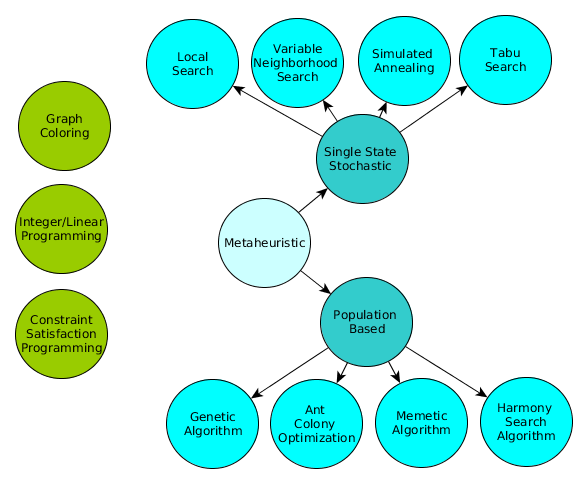
\includegraphics[scale=0.5]{./Figures/DataStructures/yED/techniques.png}
	\rule{35em}{0.5pt}
	\caption[Techniques Applied to the University Timetabling Problem]{Techniques Applied to the University Timetabling Problem} 
	\label{fig:techniques}
\end{figure}

Lewis \citep{lewis2008survey} distinguish approaches based on how the algorithms attempt to solve the two kind of constraints, i.e, hard and soft constraints. Regarding this matter, they usually fall into one of the two categories:
\begin{itemize}
	\item{\textbf{One-Stage Optimization Algorithms}} - The satisfaction of both hard and soft constraints is attempted simultaneously. In this case the violation of hard and soft constraints is allowed and the quality of a solution is measured through a typical weighted sum function, where the penalties for hard constraints are much higher when compared to violations of soft constraints. 
	\item{\textbf{Two-Stage Optimization Algorithms}} - The satisfaction of soft constraints is only attempted once feasibility is found, i.e., all of the hard constraints are solved. This has the immediate advantage of only considering weights for soft constraints and applying search techniques only in feasible areas, i.e, using classical search improvement procedures to move from old solutions to better solutions.
\end{itemize}

Carter and Laporte \citep{recent_dev_patat} extends this idea and also consider the existence of constructive heuristics, i.e, algorithms where sequential assignments are made while preserving feasibility, until is no longer possible to make assignments (due to violations). Then some backtracking procedures are applied in order to undo the changes and restart the sequential assignment process.

The next list shows a survey of related works under the categories presented in Figure \ref{fig:techniques}:

\paragraph{\textbf{Graph Coloring}} - The problem of coloring a graph with a set of colors such that no two adjacent vertices share the same color is a classic assignment problem. De Werra \citep{introduction_timetable} used this technique to solve the class-teacher timetabling problem. Basically, he described a bipartite multi-graph in which the nodes are the teachers and the classes and the edges represent a relation between a teacher and a class. Thus, two nodes may be linked by a number of parallel edges, depending on how many classes involving a teacher and a class are there. The problem is then reduced to finding an assignment of one among \textit{p} colors (timeslots) to each edge in such a way that no two adjacent edge share the same color. Another way of stating the problem is that of finding a set of \textit{n} matchings, attributing the same color to all the edges of the same matching (by definition, in a matching there are no adjacent edges) such that the final graph does not have adjacent edges with the same color. De Werra showed previously that is possible to find such matchings using network flow techniques \citep{deWerra}. 
	Figure \ref{fig:bipartite} despises this situation.\par
	  \begin{minipage}{\linewidth}
            \centering
            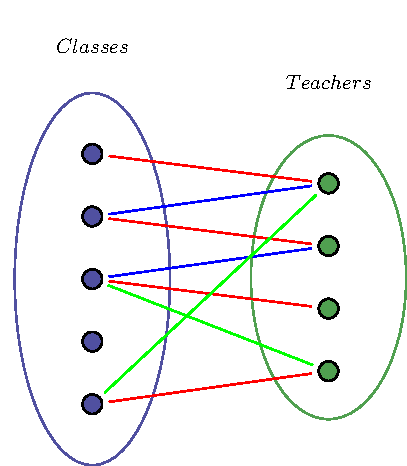
\includegraphics[scale=0.7]{./Figures/tkiz/bipartite.pdf}
            \captionof{figure}{Bipartite colored matching}
            \label{fig:bipartite}
        \end{minipage}
By using the graph coloring, Karich and Bahurmoz \citep{peter_karich},\citep{bahurmozhungarian} are able to assign events to rooms and time slots efficiently. Essentially, they use the Hungarian algorithm to find perfect matchings, i.e, matchings that minimize certain costs. The Hungarian algorithm is an algorithm that solves the assignment problem in polynomial time and is used to achieve perfect matchings that minimize the assignment costs. In this case the costs may be related to the quality of associating an event to a room or to a time slot.
    The most simple timetabling problem can be converted to a graph coloring, by considering each vertex as an event and edges representing conflicts (e.g.: cannot be assigned in the same time slot). Each color represents then a time slot and the problem is now to find an assignment of colors to vertices that used no more than the available colors. Another way of seeing the problem is to determine the minimum number of colors needed in order to avoid collisions between events, but unfortunately it is also an NP-hard problem. Nearly all timetabling problems have this underlying graph coloring problem.

\paragraph{\textbf{Integer/Linear Programming}} - Linear programs are methods used for optimizing outcomes of mathematical models, i.e, maximizing or minimizing costs. Usually, there is an objective function to be maximized or minimized. This function is also subject to some constraints usually expressed in the form of mathematical inequalities. When only integers are allowed for the values of the variables, it is called integer programming. A variant commonly used in solving timetabling problems is called 0-1 integer programming where the variables have binary values. For instance, Daskalaki and Birbas \citep{daskalaki2005efficient} developed a two-stage relaxation procedure to solve efficiently an 0-1 integer formulation of the problem. In their work, some hard constraints are relaxed (not considered) in the first stage and recovered in a second stage. In terms of formulation, they reuse the work performed in \citep{daskalaki2004integer} and they consider the possible assignment of a lecture, taught by a teacher to a set of students, scheduled in a period of day and in a classroom as a single variable that may have the value 1 (the assignment is performed) or 0 (the assignment is not performed). They later define an objective function subject to a set of formulated constraints and this optimization helps minimizing the total cost of the assignments. A downside of this approach is that introduces too many variables as the problems grows in size. On the other hand, it brings a great flexibility in terms of adapting the constraint formulations and the objective function to different requirements of different institutions.

\paragraph{\textbf{Constraint Satisfaction Programming}} - Timetabling problems may be modeled as set of clauses in which each clause has a body with constraints. Besides a set of discrete variables with discrete domains are also defined. Therefore it is possible to formulate a combinatorial problem such assigning events to time slots in terms of variables and their domains and a set of constraints that constraint the assignment of values to these variables. In constraint satisfaction programs, the objective is to find a set of values that satisfy a set of constraints. Usually this technique is followed by \textit{"forward checking"} which allows to determine the effects of assigning a value to a variable. This means that each time a variable is chosen, every other possible  assignment from another variable that is not consistent with that new assignment is eliminated from the respective domains. This brings an advantage because it decreases the search space. Besides, CSP programs have the logic separated from the control, i.e, the declaration of variables and constraints is separated from the information regarding the search strategies to follow. In fact, the university of Leeds \citep{leed_clp} developed a Prolog system based on Constraint Logic Programming (an application of logic programming languages to CSP).

\paragraph{\textbf{Local Search}} - Local search techniques consider solutions that move in the search space by exploiting several different neighborhoods. Usually, the search starts in an initial solution and iterates over the search space, steping from one solution to one of its neighborhoods. Therefore, neighborhoods are core structures of this approach and a good definition of a set of operators that create neighborhoods are usually an important part of the process. Each neighborhood is obtained by applying small "changes" called moves to solutions. Di Gaspero and Schaerf \citep{di2003multi} performed an extensive study of neighborhood structures applied to the timetabling problem. They investigate three main kind of neighborhood combinations:
	\begin{itemize}
		\item Neighborhood Union - For example, two basic resources in timetabling are time slots and rooms. Thus, by simply changing a room of a lecture or a time slot of a lecture two new neighborhoods are defined. The union operator, at each iteration of the search procedure, performs one of these moves.
		\item Neighborhood Composition - In this case, an ordered sequence of moves belonging to different neighborhoods is performed.
		\item Token-ring search - This technique performs a circular search through all the neighborhood operators and it always stars from the best solution found in the previous search.
	\end{itemize}
	Another common technique used is the Iterated Local Search and Roosi-Doria et al. \citep{rossi2003comparison} used this technique where small perturbations are made to the timetables in order to search in new promising areas. 

\paragraph{\textbf{Variable Neighborhood Search}} - Variable neighborhood search usually uses more than one neighborhood structure where those structures may change during the local search. Abdullah et al. \citep{abdullah2005investigation} use an acceptance criteria similar to simulated annealing but without a cooling schedule. The motivations was to search new points of the search space. In terms of neighborhood moves, they implemented twelve different operators in which some of them simply move a lecture (obtained from a random sample of varying size of assigned lectures) to a new feasible time slot. The algorithm followed an iterative three stage approach where first a random solution is obtained followed by a local search and then the new solution is accepted based on a acceptance criteria. As highlighted by the authors, the order of neighborhoods that gave the best results was when the neighborhood structures were ordered in an increasing size, i.e, with a bigger number of possible moves. This way solutions could go smoothly from local searches to more global searches.
  

\paragraph{\textbf{Simulated Annealing}} - Simulated annealing is a search strategy inspired  in the slow annealing process in metallurgy. The difference from a simple Hill Climbing algorithm is in its decision of when to replace a solution, i.e, a newly tweaked solution may be accepted even if it is worse than the current solution, according to a certain probability. This probability is controled by a parameter called temperature and the rate at which this value is changed is called the cooling schedule. Aycan and Ayav \citep{aycan2009solving} use a simulated annealing approach to solve the timetabling problem.  This approach is a very problem dependent because it needs a suitable cooling schedule and good neighborhood structures. In order to create neighborhoods, random lectures were given new time slots or two lectures had their time slots swapped or two random lectures were assigned to two new random time slots.

\paragraph{\textbf{Tabu Search}} - Tabu search is a search procedure that keeps an history of moves that led to better solutions (a tabu list), i.e, usually a solution that is obtained by applying repeated moves from the past is avoided, preventing cycles. This avoid locking solutions in suboptimal regions, like local minima. Tabu search uses a local or neighborhood search procedure to iteratively move from one potential solution to an improved solution in the neighborhood. Tabu search provides intensification and diversification, i.e, it examines thorough the neighborhood of good quality solutions and force the search to unknown regions. For the past ten years, Alvarez-Vald{\'e}s et al. \cite{alvarez2001tabu}  have applied tabu search methods in timetabling problems. They use tabu lists of varying lenght, giving better results than static length lists. Another simple criterion that usually works well, is the aspiration criterion where sometimes, a not so good solution may be accepted, ignoring the moves in the tabu list. 

\paragraph{\textbf{Genetic Algorithm}}- Genetic algorithms are inspired in biological mechanisms and reuse similar concepts such as a population, selection of the fittest when subject to an objective function, recombination and mutation where diversity is created and slowly increases the quality of the population in the long run. Common solution representations include encoded numeric arrays where each cell represents the time slot where each event is going to take place. The evolutionary approach used by Roosi-Doria et al. \citep{rossi2003comparison} used this representation with an additional matching algorithm to determine the best suitable room. Such simple representations allows to use crossover and mutation operators (for example, inheriting, in a uniform way, time slots from the parents or a simple swap of events). Usually these procedures are followed by local search techniques in order to improve the quality of the solutions. Carrasco and Pato \citep{carrasco2001multiobjective} developed a multiobjective genetic algorithm that deals with two main objectives: the minimization of both types of constraints and the minimization of conflicts between teachers and classes, i.e, the competing aspects of the soft constraints. The chosen representation was a matrix of time slots per rooms where each cell stored the lecture event currently taking place. The population then evolved over the generations  by applying genetic operators. An interesting fact is that the algorithm also kept a secondary elitist population where the best candidates were saved for the next generation in order to avoid the loss of high-quality solutions. 

\paragraph{\textbf{Ant Colony Optimization}} - Ant colony optimization is another family of optimization algorithms inspired by pheromone-based strategies of ant foraging. The main idea is that ants move randomly in order to find food, while depositing pheromones, leaving a track that becomes stronger as others ants find this track and keep depositing pheromones. There is also a constant phenomenon of evaporation that slowly erases the left pheromones. Roosi-Doria et al. \citep{rossi2003comparison} were the first to apply such technique for a timetabling problem. The method is an iterative process where each ant builds an assignment and keeps a matrix of pheromone values (Time slots $\times$ Events). In order to construct an assignment, an ant chooses the next event from an ordered list and a time slot for that event, based in probabilistic heuristics. Then, it updates the corresponding cell in the pheromone matrix. The probabilistic heuristics were guided by taken into account potential constraint violations and a "rating" of that assignment given by the value of the current pheromone. Besides the pheromones values were constantly being updated after each event assignment and in the end of the iterative process. The iterative process would then keep running for a defined period of time. 

\paragraph{\textbf{Memetic Algorithm}} - Just like genetic algorithms are inspired in biological evolution, memetic algorithms are inspired in the evolution of memes, i.e, symbols or cultural ideas that are transmitted over the generations and may also evolve. The main difference between genes and memes is that memes can be improved by the individual, i.e, memetic algorithms are basically evolutionary algorithms with local optimization techniques. Rossi-Doria and Paetcher \citep{rossi2004memetic} use a classical genetic algorithm with genetic operators (recombination and mutation) to evolve a population but in the end of each iteration, they perform additional local searches. In another work, Paetcher et al. \citep{paechter1996extensions} detail a system in which the local search mechanism consist in suggestion lists of possible time slots, one for each event. The list of events is also permuted in order to place first events with a fewer possibilities first. A mechanism called \textit{searchspec} consists in trying to place an event in each time slot of its suggestion list and if the move is successful, the time slot is moved to the top of the list, improving the memetic material. Other recombination operators are also applied, ensuring that quality ideas are passed over the generations (ancestral memory). 

\paragraph{\textbf{Harmony Search Algorithm}} - Harmony search algorithms are inspired in the process of improvised creation of beautiful harmonies by musicians. Musicians improve the pitches from their musical instruments achieving a pleasant harmony after repeated sessions. In a similar way, a set of decision variables are assigned with values and after repeated iterations, an optimal solution may be found according to an objective function. There are many similarities with genetic algorithms because this technique stores a set of vector variables (solutions) with possible values assigned, just like a typical population, but in this case is called harmony memory. Just like genetic operators, there are operators that change the values of the variables. Finally, by an iterative process the worst vector variable (in terms of quality) is continually replaced by a newly improvised vector, if this one is better. Al-Betar et al.\citep{al2012university} adapted this search procedure to the timetabling problem, by representing a solution as a vector of \textit{n} event variables, where each value maps a room and a time slot (according to a mapping function) for the event represented by the index position. 

\subsection{Standard Formats and Benchmarks}

Usually many different methods are developed to solve the timetabling problems. However, these methods are usually very problem-specific and are only used in a particular institution or research group and are rarely compared with each other. Thus, a problem arises when trying to compare existing methods and determining the best approaches. If a method is simple enough to reproduce, this does not represent much of a problem, but as the complexity of the constraints and techniques grows, comparisons become much harder.\\
Many formats have been developed in order to express in a clear and precise way real-life timetabling problems. Although, the comparison of results and exchange of data between researchers is a difficult process because each one has its own way of formulating the problem. Therefore, the need for a standard format that allows easy exchange of data and testing of algorithms on standards benchmarks have become urgent along the years. Burke et al. \citep{burke1998standard} proposed a functional format for expressing the timetabling problem in a mathematical form. The proposed format was intended for storing data centrally, allowing different researchers to exchange data via this central format.
Currently, the WATT research group also provides datasets from different universities and tools (solutions, verificators, generators and libraries) \footnote{\href{http://www.cs.nott.ac.uk/~yxb/TTdata/}{http://www.cs.nott.ac.uk/~yxb/TTdata/}}.
A good example that promotes the sharing of datasets and testing of algorithms on benchmarks is the International Timetabling Competition \footnote{\href{http://www.utwente.nl/ctit/hstt/itc2011/welcome/}{http://www.utwente.nl/ctit/hstt/itc2011/welcome/}}. The purpose of this competition is for participants to submit algorithms able to solve real world instances of the timetabling problem and then be compared against each other using existing benchmark data. In a very realated work, Roosi-Doria et al. \citep{rossi2003comparison} studied the performance of five different metaheuristics (Evolutionary Algorithms, Ant Colony Optimization, Iterated Local Search, Simulated Annealing and Tabu Search). Both one-stage and two-stage approaches were tried and in general, algorithms with a two-stage approach performed better. Although the performance of the metaheuristics are highly dependent of the context in which they are used, i.e, the solution representation used, neighbourhood search structures, constraints, techniques that used iterated local search offered good results and in many cases outperformed the others.

\section{Technological Overview}

In the following sections we present a small survey of practical approaches currently in use at universities. The technical details of these approaches were gathered from published conference papers, namely the PATAT conference
\citep{leed_clp, purdue_patat_2006, bullet_paper, thor, distributed_timetabling, online_tt_patat2010, diamant}.  

\subsection{Automated Timetabling at the University of Leeds}
At the University of Leeds, the informatics department developed a timetabling engine with a central database capable of storing all of the required information. The implemented algorithm followed an approach based on constraint logic programming \citep{leed_clp}. The used constraints were  formulated in a CLP program.
The implementation consists in several modules that work together. Figure \ref{fig:leeds_workflow} shows the implemented workflow.
\begin{figure}[htbp]
	\centering
		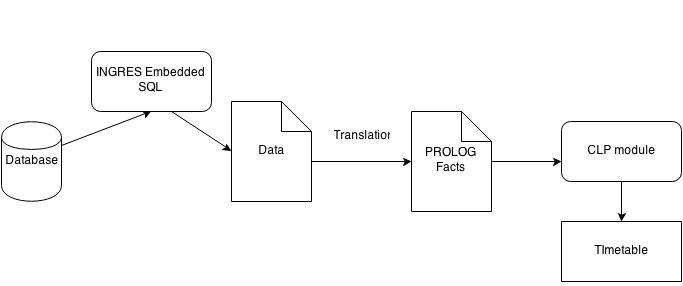
\includegraphics[width=\textwidth]{./Figures/leed_workflow.png}
		\rule{35em}{0.5pt}
	\caption[Implementation workflow of a CLP based system]{Implementation workflow of a CLP based system}
	\label{fig:leeds_workflow}
\end{figure}
 
A SQL script is used to extract the required data from the database. This data is then translated to PROLOG facts. These facts represent the formulation of the problem and will be read by the CLP module. This CLP module is then responsible for generating the timetables.

\subsection{Automated Timetabling in the Purdue University}
In the University of Purdue, a system is being implemented with the main goal of assisting the academic timetablers in constructing a feasible and good timetable \citep{purdue_patat_2006}. The university has large dimensions (9,000 classes, 570 rooms, and 39,000 students) and thus it was necessary to come up with a scalable solution that could deal with the problem.

The developed system consists on 2 different modules:
\begin{itemize}
	\item User Interface - A web-based client-server application written in Java (J2EE) and Hibernate/Oracle Database as the persistence components.
	\item Solver - An engine capable of generating schedules using a Iterative Forward Search approach. This technique is a mixture between local search methods and backtracking because it operates over feasible (not necessarily complete but with all constraints satisfied) solutions.
\end{itemize} 

In terms of features of the application we present a list of interesting aspects:
\begin{itemize}
	\item Interactive changes - If a user wants to change a given class, the interface would provide a list of possible and feasible suggestions (based on a search of limited depth) and the reachable solution cost. The system could also relax some constraints in order to give more freedom to the user when choosing, for example, a room for the class, allowing the user to choose a conflicting room. Of course, if this were the case, all the conflicting events (also shown) would be unassigned. 
	\item Data Consistency - The solver is capable of checking the input for inconsistencies and informing the user about the problem.
	\item Data Management - Possibility of defining preferences and deducing new constraints from these preferences. 
\end{itemize}


\subsection{Bullet TimeTabler Education}
\label{bullet_algorithm}

In Portugal, a company called Bullet Solutions developed a timetabling engine \citep{bullet_paper}.
The followed approach is based on some important principles:
\begin{itemize}
	\item An initial difficulty is to create an initial feasible solution. Therefore, the focus should be on find good methods that allow finding feasible solutions.
	\item The solutions should be found in due time. Therefore, it is important to achieve methods that can quickly cover many areas of the search space. 
\end{itemize}

Given these two principles, the developed algorithm consisted in the following two steps:
\begin{itemize}
	\item Building of an initial solution.
	\item Optimizing the initial solution applying some heuristics. 
\end{itemize}

Initially there is a ordered list of events to be scheduled. The order of criterion is basically the urgency of each event. The urgency of an event is defined by factors like the number of available time slots, the number of available rooms (the lower, the most urgent) or the degree of dependency (through constraints) with other events (the higher, the most urgent).\\ 
This list also contains some redundant events (ghost events) that will not be scheduled in order to increase the flexibility of the algorithm. These ghost events represent the many possible combinations between teachers and turns of a subject. This happens because the algorithm does not consider the association between teachers and their respective turns. In case there are more than one teacher for a given subject, and that subject is taught in more than one turn, there is many possible combinations teacher-turn. Of course if a given event is scheduled, all his complementary ghost events are no longer valid.

After the first feasible solution is found (all events scheduled with hard constraints satisfied), a local search is applied to the solution in order to increase its quality. This search is performed in the neighborhood of the solutions and uses two search operators:
\begin{itemize}
	\item Operator 1 - This operator chooses an event and analyses potential new places to be scheduled. The event may then be moved to these new locations or the events occupying these destination places may be swapped with original event, if possible.
	\item Operator 2 - This operator differs from the first in the swap operation. The destination place is not restricted to the location of the other event. Instead, new locations are possible. 
\end{itemize}

Besides, the software also tries to optimize the use of spaces, i.e., it changes the assigned classrooms in order to optimize the space usage.



\subsection{The THOR System}

The THOR system \citep{thor} was developed by ISEL (Lisbon Institute of Engineering) and is currently commercialized by the company F++, Informática e Serviços. The main objective was to solve the problem of timetabling in Portuguese institutions and to give support to different levels of education (basic, higher, academic,etc). \\
The basic scheduling unit considered is a lesson. A lesson is a triple (T,C,S) in which T is a subset of teachers, C is a subset of classes and S is a subset of subjects. Therefore, a lesson may be simple (when there is only one class and only one subject) or compound (there is more than one class and more than one subject). A compound lesson may have many classes associated with a single subject or a given class associated with many subjects.

The authors made no clear no clear distinction between hard and soft constraints. This problem was solved assigning weights to each constraint and thus allowing different schools assigning different values.


The implementation of the system was divided into three main modules:
\begin{itemize}
	\item A Graphical User Interface - Several forms where it is possible to enter school data and manipulate the schedules.
	\item An automatic scheduler - Developed in C++ using an object oriented approach. The scheduler is capable of following two approaches: An iterative algorithm and a heuristic constructive algorithm. In order to achieve fast evaluations between two neighbor solutions, the cost function is computed incrementally, i.e., the computed value is the difference change in cost between the old solution and the new solution. 
	\item A relational database - Implemented in Microsoft Access.
\end{itemize}

According to the authors, this implementation is currently in use in more than one hundred national schools.

\subsection{A framework for Distributed Timetabling}

At the University of Erlangen-Nuernbergat, efforts have been made in order to come up with a framework that can support all of the timetabling algorithms with optimal parameter settings, \citep{distributed_timetabling}. This requires that all of the algorithms share the same interface which allows the framework setting and optimizing the parameters in runtime and running different algorithms. 

\begin{figure}[htbp]
	\centering
		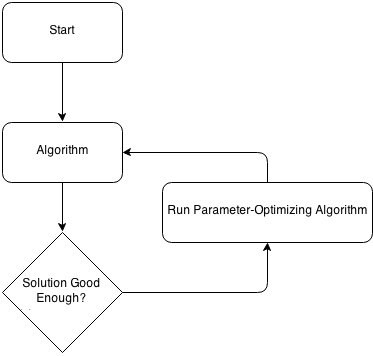
\includegraphics[scale=0.55]{./Figures/distributed_timetabling.png}
		\rule{35em}{0.5pt}
	\caption[Simplified model of a distributed timetabling for timetabling]{Simplified model of a timetabling framework}
	\label{fig:distributed_timetabling}
\end{figure}

Figure \ref{fig:distributed_timetabling} presents the framework model. The box algorithm represents any algorithm that is ready to compute a solution and if the resulting solution is not good enough (according to some criteria) a parameter-optimization-algorithm is run in order to find a better configuration. This process can iterate many times until a good solution is found.\\
This framework supports a wide range of algorithms such as Evolutionary Algorithms, Branch-and-Bound, Tabu Search and Simulated Annealing methods, runs on Windows and Linux Platforms and is implemented in JAVA, which consists of a server (JBOSS) a middle-ware (Hibernate) and a persistence engine (SQL-database). The computations are also distributed over the network using JAVA RMI technology.

\subsection{On-line Timetabling Software}
Florent Devin and Yannick Le Nir \citep{online_tt_patat2010} developed a user friendly solution using advanced technologies in the area of Rich Internet Application (RIA) and constraint programming in order to compute the timetable.


The constraints are then modeled in a constraint programming model, which requires specifying the variables, domains and constraints that constraint the assignment of variables and is implemented in swig-prolog. Web services are used to communicate with the user interface (implemented using RIA) and the communication with the database is made using a classic ODBC. 

The user interface is developed using RIA, with the ZK JAVA framework. RIA is a technology that does not require any installation on the client and it is inherently distributed, allowing users of the timetabler engine to specify constraints in a rich interface. An interesting aspect of this system is the distinction of roles, i.e., there is the normal user and the administrator. The normal user may suggest and add new constraints and the administrator will accept or refuse these new constraints. In this case, an user is someone who is allowed to submit new constraints to his own timetable.\\
In terms of persistence of the data, it is used a central shared database which is accessible by the RIA interface and the Prolog engine through Hibernate and a classical ODBC, respectively. \\
This system shows a modern approach using the advantages of RIA for data acquisition and constraint programming to compute the timetables.

\subsection{The Diamant System}

At University of Sherbrooke, the research group developed a open-source system \footnote{\href{https://github.com/gonr1001/diamant}{https://github.com/gonr1001/diamant}} capable of automatically produce class and exam timetables \citep{diamant}. Essentially the system is divided into two parts:
\begin{itemize}
	\item A module that reads data from the database and formats it according to Diamant requirements (e.g., events, students, instructors, rooms, etc).
	\item A module capable of producing timetables. This module is implemented in JAVA and follows the MVC pattern. The model contains the set of events, instructors, rooms, students and the current state of the timetable. The views give the visual representation of the sets and the timetable and reflect any changes made to the model. The controllers create a bridge between the views and the model. They control the actions sent from the view to the model, updating both parts. It is important to note that this implementation follows the open-closed principle, which means the software entities (the original classes, methods) are closed to modification but open for extension. This design pattern allows customization without modifying the source code. This system also encapsulates the algorithms with interfaces and thus allowing different implementations. 
\end{itemize}

The fact that this system is extensible, allows institutions to adapt the software to their specific needs.
%----------------------------------------------------------------------------------------
\subsection{Summary of the Features}

The presented solutions share some common characteristics and differ and innovate in others.
Table \ref{tab:summary_tech_art} shows a summary of the features presented and how these relate with the timetabling engine.

\begin{table}[H]
\centering
\resizebox{\textwidth}{!}{%
\begin{tabu}{|c|c|c|c|c|c|c|c|c|}
\hline
\multirow{2}{*}{\backslashbox{Feature}{System}} & \multirow{2}{*}{Leeds} & \multirow{2}{*}{Purdue} & \multirow{2}{*}{Bullet} & \multirow{2}{*}{THOR} & \multirow{2}{*}{\shortstack{Distributed\\ Timetabling}} & \multirow{2}{*}{\shortstack{On-line\\ Timetabling}} & \multirow{2}{*}{Diamant} & \multirow{2}{*}{\shortstack{Timetabling\\ Engine}}\\

	& & & & & & & &  \\
\hline
	Persistent Database & \ccheck & \xcheck & \xcheck & \ccheck & \ccheck & \ccheck& \ccheck & \ccheck \\
\hline
	User Interface & \xcheck& \ccheck & \ccheck & \ccheck & \xcheck & \ccheck & \ccheck & \xcheck\\
\hline
	Solver & \ccheck & \ccheck & \ccheck & \ccheck & \ccheck & \ccheck & \ccheck & \ccheck \\
\hline
	Interactive Changes & \xcheck & \ccheck & \ccheck & \ccheck& \xcheck & \xcheck&\xcheck & \xcheck\\
\hline
	Input Validation & \ccheck & \ccheck & \ccheck & \ccheck & \ccheck & \ccheck & \ccheck & \ccheck \\
\hline
	Flexibility in Preferences & \ccheck & \ccheck & \ccheck & \ccheck& \ccheck & \ccheck & \ccheck & \ccheck \\
\hline
	Distinction of Roles & \xcheck & \xcheck & \xcheck& \xcheck & \xcheck & \ccheck & \xcheck& \xcheck \\
\hline
\end{tabu}%
}
\caption[Summary of the software features]{Summary of the software features}
\label{tab:summary_tech_art}
\end{table}



% Chapter 4
%http://www.cs.iit.edu/~oaldawud/CS487/project/software_design_specification.htm


\chapter{Architecture of the Engine}
%\epigraph{A fancy quote.}{Me}

\label{engine} % For referencing the chapter elsewhere, use \ref{Chapter2} 

\lhead{Chapter 4. \emph{Architecture of the Engine}} % This is for the header on each page - perhaps a shortened title

This chapter describes the architecture of a possile timetabling engine. It describes internal data structures, a data model and a possibility for a timetabling algorithm. Other important topics like the evaluation function and computational complexity are also discussed.

\section{Data design}
Data design is an important step in software development. It is a process that gives a good overview of how the data will be organized and accessed. Characteristics like simplicity, fast data access, extensibility and maintainability were kept in mind when designing such structures.    
\subsection{Solution Representation}


Usually, in a formal definition of the University Class Timetabling Problem, we have a set of \textit{n} events, a set of \textit{m} rooms and a set of \textit{t} available time slots. This means that we have \textit{m} $\cdot$  \textit{t} possible places where to schedule the events and it is easy to see that the problem is only solvable if \textit{m} $\cdot$  \textit{t} $\geq$ \textit{n} .\\
Since we know that we cannot have two different events with same combination of a room and a time slot, a possible representation for a timetable is a  matrix in which rows represent the rooms and the columns represent the time slots. Besides, this representation does not allow the scheduling of different events in the same room, and thus solves an important constraint and reduces drastically the search space. This brings an advantage against other possible representation that do not take this fact into account, for example, an array of size \textit{n} where each cell indexes a time slot and a room. In fact, if we did not consider this information and that each event occurs in a single time slot, the total number of ways of assigning \textit{n} events to \textit{m} $\cdot$ \textit{t} places would be:

\begin{center}
$(m \cdot t)^{n}$
\end{center}

On the other hand, this representation reduces search space to:
\begin{equation}
\label{comb_assign}
\begin{split}
\binom{m \cdot t}{n} \cdot n! & = \frac{(m \cdot t)!}{n! (m \cdot t - n)!} \cdot n! \\
& = \frac{(m \cdot t)!}{(m \cdot t - n)!}
\end{split}
\end{equation}

In Eq. \ref{comb_assign}, the first factor represents the arrangement of these $n$ events over the \textit{m} $\cdot$ \textit{t} places and the second factor of the first member represents the possible permutations of an assignment.
Figure \ref{fig:solution_representation} shows a very simple scenario with 2 week days (represented by different colors), 10 events and 10 rooms. Each cell has the id of the scheduled event and may have only one. Besides, there may be events of longer duration occupying more than one cell.

\begin{figure}[t]
	\centering
	\resizebox{\textwidth}{!}{
	    \input{./Figures/tkiz/solution.tkiz} 
	  }
	\rule{35em}{0.5pt}
	\caption[Solution representation]{Solution representation} 

	\label{fig:solution_representation}
\end{figure}

In order to restrict the search space even more, we use additional information mainly regarding constraints and availabilities. 
}
Figure \ref{fig:search_space} shows a representation of the search space for this problem. The green areas represent the feasible solutions and the red areas represent solutions that are forbidden (unfeasible) because of additional constraints.

\begin{figure}[t]
	\centering
	    \input{./Figures/tkiz/search_space.tkiz} 
		\rule{35em}{0.5pt}
	\caption[Search Space]{Search Space} 
	\label{fig:search_space}
\end{figure}


\subsection{Data Structures}

In order to maintain information regarding constraints some auxiliary data structures may be used. Besides, additional data regarding the current state of the solution may also be  kept in memory because it helps to speed up constraint violations checks. In this section, we introduce the data structures used and in the next section we make a comprehensive review of the operations that make use of these structures and also a time and space complexity analysis. \\
Usually, precedences happen between events lectured by the same teacher(s). Thus, it is useful to keep in memory information regarding the current order of assigned events for each teacher. Figure \ref{fig:teacher_events_timeslots} shows a possible representation of this information. The head nodes store the teachers ids and the lists store the event ids. For example, in Figure \ref{fig:teacher_events_timeslots} there are five teachers and for instance the first teacher has the events 2 and 5 assigned.
Figure \ref{fig:precedence_matrix} shows a matrix that stores information about precedences between events. Precedences may be hard or soft, for example, a theory lecture event must happen before a practical event but between practical events, this constraint may be soft. Each  cell with 1 represents a hard precedence, whereas 2 represents soft precedences between events. 

\begin{figure}[th]
	\centering
	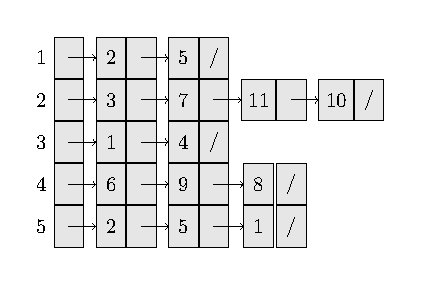
\includegraphics[scale=0.95]{./Figures/tkiz/teacher_schedule.pdf}
	\rule{35em}{0.5pt}
	\caption[Current order of teacher events]{Current order of teacher events} 
	\label{fig:teacher_events_timeslots}
\end{figure}
\

 Figure \ref{fig:distance_matrix} shows a distance matrix where each cell represents the minimum required temporal distance between two events. For example, in Figure \ref{fig:distance_matrix} the events 3 and 5 should have a temporal distance of 5 time slots. In order to quickly check if the distance between two events is being respected, an associative array that stores the beginning time slot of each event is useful because one only needs to compute the distance between two events and compare it with the information in the distance matrix. Each index represents a single event and maps the first time slot at which an event begins.\\

\begin{figure}[thp] 
  \label{ fig7} 
  \begin{minipage}[b]{0.5\linewidth}
		\centering
		\input{./Figures/tkiz/precedences.tkiz}
		\caption[Precedence matrix]{Precedence matrix}
		\label{fig:precedence_matrix}
		\vspace{4ex}
  \end{minipage}%%
  \begin{minipage}[b]{0.5\linewidth}
        \centering
        \input{./Figures/tkiz/distances.tkiz}
		\caption[Distance matrix]{Distance matrix}
		\label{fig:distance_matrix}
    \vspace{4ex}
  \end{minipage} 
  \begin{minipage}[b]{0.5\linewidth}
	    \centering
		\input{./Figures/tkiz/restrictions.tkiz}
		\caption[Constraint matrix]{Constraint matrix}
		\label{fig:constraint_matrix}
		\vspace{4ex}
  \end{minipage}%% 
  \begin{minipage}[b]{0.5\linewidth}
        \centering
		\input{./Figures/tkiz/pa.tkiz}
		\caption[Teacher availability]{Teacher availability}
		\label{fig:teacher_matrix}
    \vspace{4ex}
  \end{minipage} 
    \begin{minipage}[b]{0.5\linewidth}
        \centering
		\input{./Figures/tkiz/ra.tkiz}
		\caption[Room availability]{Room availability}
		\label{fig:timeslot_room_matrix}
    \vspace{4ex}
  \end{minipage} 
   \begin{minipage}[b]{0.5\linewidth}
        \centering
		\input{./Figures/tkiz/ru.tkiz}
		\caption[Room usage]{Room usage}
		\label{fig:room_usage}
    \vspace{4ex}
  \end{minipage} 
\end{figure}

Figure \ref{fig:constraint_matrix} represents multiple constraints encoded in a single matrix. One for contiguous events, two for events occurring in different days, three for events occurring in different time slots, four for overlapped events, five for events starting at the same time and finally six for events occurring in the same day. Once again, an associative array is useful because it allows to quickly locate the events and then perform small computation checks.\\
Figure \ref {fig:teacher_matrix} shows a matrix with the teacher availabilities encoded. This matrix serves only for fast availability checks. Essentially, a teacher may be available in a time slot (0) or recently unavailable (1), i.e, during the search, this value may become 0 again. It is important to note that this matrix translates the actual state of the teacher availabilities according to the current solution, that is, the current teacher availability that may change in the future. This matrix is useful when trying to place a teacher in a time slot. The teacher will only be placed if this matrix allows it (value 0 in the corresponding time slot). It is important to remember that each teacher has an ordered list of preferential time slots and it is represented with a similar structure shown in Figure \ref{fig:teacher_events_timeslots}. In this case, the lists contain time slots. The search starts in this list, and for each preferential slot, it checks the matrix and thus avoiding an important restriction of not placing teachers in non desired time slots and in unavailable time slots.\\
As explained in the Chapter \ref{current_process}, there is an order in which the departments create the schedules. Therefore, it is natural that certain rooms are always unavailable in certain time slots (because they have scheduled lectures from another department). In order to take into account this information, the matrix represented in Figure \ref{fig:timeslot_room_matrix} may be used. Similar to the teacher availabilities, zero values represent available time slots and cells with the number one represent unavailable time slots. The structure presented in Figure \ref{fig:room_usage} is useful to measure the room usage. Each time an event is inserted in the time table, the value of the cell is incremented (different events may belong to the same subject). The final value for each subject or teacher (in the last row) is the number of rooms currently in use. For example, in Figure \ref{fig:room_usage} the teacher with the id 7 is currently using 2 different rooms (2 times in the room 5 and one in room 6). On the other hand, the same kind of structure (but in a different matrix) may also encode the room usage by subjects, following the same idea.

\begin{figure}[t]
	\centering
	    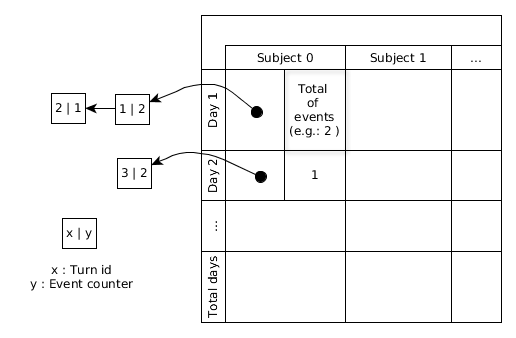
\includegraphics[scale=0.45]{./Figures/DataStructures/yED/cp_tracking_distribution.png}
	\rule{35em}{0.5pt}
	\caption[Structure to keep track of the distribution of events]{Structure to keep track of the distribution of events} 
	\label{fig:distribution_events}
\end{figure}

Figure \ref{fig:distribution_events} represents a structure useful to count the distribution of a subject over the week. For each day and for each subject, each time an event is inserted, the corresponding node is incremented. Therefore, each node counts the number of events from a given turn from a certain subject in a certain day, simulating the point of view of a student who attends classes from that turn. With this structure updated, it is easy to compute the distribution of events (number of days) from a subject (from the point of view of the student). One only needs to check how many days with non zero values exist (for each subject), represented in the example by the final row. For instance, in Figure \ref{fig:distribution_events}, in the first day, the subject with id 0 is having classes from turn 1 and 2, and classes from turn 3 in the second day.\\

\begin{figure}[h]
	\centering
	    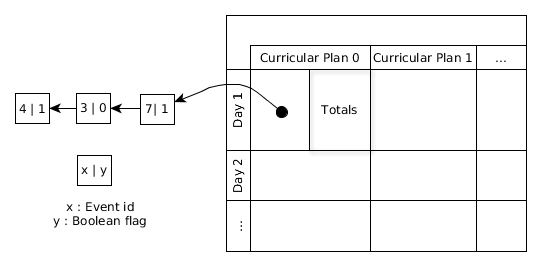
\includegraphics[scale=0.45]{./Figures/DataStructures/yED/cp_tracking.png}
	\rule{35em}{0.5pt}
\caption[Generic structure to keep track of events]{Generic structure to keep track of events} 
	\label{fig:tracking_cp_events}
\end{figure}

In order avoid full table scans, there is the need to maintain a generic structure that keeps track of the events of each curricular plan, in each day is useful. Figure \ref{fig:tracking_cp_events} shows a simple example of this structure. Besides it is also useful to store additional information about the current state of the solution. In the example, for each cell in the matrix there is a sorted list of events happening on that day. There is also information that may be extracted from that current list and is stored as a list of values represented in the Figure \ref{fig:tracking_cp_events} by totals. These totals are important when analyzing constraints because they give immediate feedback that is useful to decide if certain constraints are met. Another important aspect of this structure is that avoids double countings, i.e, if certain constraints do not consider the differences between events from the same class and typology, it is important to also keep track of which events are already considered. In Figure \ref{fig:tracking_cp_events} each element from the list contains the event id and if it is already counted or not. Further explanation about this structure is explained in the next section where an analysis of the complexity of the operations is made. 

\begin{figure}[t]
	\centering
	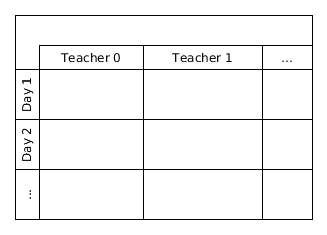
\includegraphics[scale=0.5]{./Figures/DataStructures/yED/generic_info_tracking.png}
	\rule{35em}{0.5pt}
	\caption[Generic structure to store numerical data about teachers]{Generic structure to store numerical data about teachers} 
	\label{fig:teacher_stats_track}
\end{figure}

Another useful structure to keep information about teacher is a matrix presented in Figure \ref{fig:teacher_stats_track}. Each cell of this matrix stores numerical data that changes over time and reflects some aspects from the current solution.

\section{Complexity and Performance Issues}

One of the main operations of the timetabling algorithms is to check constraint violations. Therefore, it is important to these validations to be reasonable fast, i.e, it should be avoided scanning the entire timetable when making the decision if a certain solution is feasible or not. The key idea is to increase the speed of the validations at the cost of using more memory.
\label{lab:complexity_analysis}

\begin{table}[H]
\centering
\begin{tabular}{|l|c|c|}
\hline
	Operation & Worst-Case Analysis \\
\hline
	Array lookup & $\mathcal{O}(1)$ \\
	\hline
	Matrix lookup & $\mathcal{O}(1)$ \\
	\hline
	Precedences/Distance/Constraint matrix scan & $\mathcal{O}(E^2)$ \\
	\hline
	Insert teacher event (Figure \ref{fig:teacher_events_timeslots}) & $\mathcal{O}(E)$ \\
	\hline
	Delete teacher event (Figure \ref{fig:teacher_events_timeslots}) & $\mathcal{O}(E)$ \\
	\hline
	Insert event (Figure \ref{fig:tracking_cp_events}) & $\mathcal{O}(E)$ \\
	\hline
	Delete event (Figure \ref{fig:tracking_cp_events})& $\mathcal{O}(E)$\\
\hline
\end{tabular}
\caption[Time-complexity of various operations]{Time-complexity of various operations\\ \textit{E} - Number of events}
\label{tab:complexity_operations}
\end{table}

Table \ref{tab:complexity_operations} shows the worst-case complexity of some common operations that are performed when analyzing constraints. In order to insert events in the structure presented in Figure \ref{fig:tracking_cp_events} an initial scan is needed to correctly set the flag. Then a second scan is performed to insert the new event in the correct order. On the other hand, when deleting an event, if the event was previously set with the flag 1 (meaning that this event was being counted), another event must be chosen (from the same subject) and set with a new positive flag. This involves, at most, two complete scans on this list.

Table \ref{tab:new_common_constraints} shows a set of flexible constraints, i.e., they may be considered hard or soft constraints. These constraints are essentially the same as the constraints used by the Bullet Solutions software.
It is also shown the worst case complexity for each case. The first presented complexity is applicable when a solution is being analyzed considering all of the events, i.e, the entire solution. The second is applicable to the computation of the difference between an old solution and a new one, i.e, an incremental approach where every time a new event is inserted, only the potential changes to the solution are computed and updated. This allows the solution to be always feasible because forbids invalid moves.   
\begin{table}[H]
\centering
\resizebox{\textwidth}{!}{%
\begin{tabular}{|p{10cm}|c|c|c|c|}
\hline
\multicolumn{1}{|c|}{\multirow{2}{*}{Hard / Soft Constraint}} & \multicolumn{2}{|c|}{Worst-Case Analysis } \\
\cline{2-3}   & Entire Solution & Incremental Approach\\
\hline
	Order of typologies must/should be respected (Figure \ref{fig:precedence_matrix}) & $\mathcal{O}(P \cdot E)$  & $\mathcal{O}(E)$\\
\hline
	Event A and B must/should be contiguous  (Figure \ref{fig:constraint_matrix}) & $\mathcal{O}(E^2)$ & $\mathcal{O}(E)$\\
\hline
	Event A and B must/should be overlapped (Figure \ref{fig:constraint_matrix}) &  $\mathcal{O}(E^2)$ & $\mathcal{O}(E)$ \\
\hline
	Event A and B must/should not be overlapped (Figure \ref{fig:constraint_matrix}) & $\mathcal{O}(E^2)$ & $\mathcal{O}(E)$\\
\hline
	Event A and B must/should be in different days (Figure \ref{fig:constraint_matrix}) & $\mathcal{O}(E^2)$ & $\mathcal{O}(E)$\\
\hline
	Event A and B must/should start at the same hour & $\mathcal{O}(E^2)$ & $\mathcal{O}(E)$\\
\hline
	Event A and B must/should be in the same day & $\mathcal{O}(E^2)$ & $\mathcal{O}(E)$\\
\hline
\end{tabular}%
}
\caption[Complexity of common (hard/soft) constraints used in the engine]{Complexity of common(hard/soft) constraints used in the engine.\\ \textit{P} - Number of teachers, \textit{E} - Number of events}
\label{tab:new_common_constraints}
\end{table}

In order to check if precedences are being respected, one only has to look at the current events order of a teacher. This order is stored in a structure like the one presented in Figure \ref{fig:teacher_events_timeslots}. An additional look up at the associative array (in order to obtain the beginning time slot of each event) is needed, which is a constant operation. The remaining constraints presented in Table \ref{tab:new_common_constraints} are translated into two simple lookups (per two events) to the associative array of events and the afterwards computation.\\


Table \ref{tab:new_hard_constraints} shows the hard constraints considered and their worst-case complexity. It is important to note that some constraints are excluded by definition, i.e, they are solved thanks to the chosen representations, for instance, two different events must not share the same
room and time slot or the fact that teachers are not scheduled in unavailable time slots. 
 

\begin{table}[H]
\centering
\resizebox{\textwidth}{!}{%
\begin{tabular}{|c|p{8cm}|c|c|c|c|}
\hline
	\multicolumn{1}{|c|}{\multirow{2}{*}{Point of View}} & \multicolumn{1}{|c|}{\multirow{2}{*}{Hard Constraint}} & \multicolumn{2}{|c|}{Worst-Case Analysis } \\
 &  &  Entire Solution & Incremental Approach\\
\hline
	Event & All distances between events must be respected (Figure \ref{fig:distance_matrix}) & $\mathcal{O}(E^2)$& $\mathcal{O}(E)$\\
\hline
	Student & Lunch hours for each curricular plan should be respected & $\mathcal{O}(E^2)$ & $\mathcal{O}(1)$  \\
\hline
	Student & A student cannot attend two obligatory subjects from the same curricular plan at the same time & $\mathcal{O}(E^2)$ & $\mathcal{O}(E)$ \\
\hline
	Teacher & A teacher must not be scheduled in two time slots at the same time (Figure \ref{fig:teacher_events_timeslots})& $\mathcal{O}(P\cdot E)$ & $\mathcal{O}(E)$ \\
\hline
	Teacher  & Lunch hours must be respected (Figure \ref{fig:teacher_events_timeslots}) & $\mathcal{O}(P \cdot E)$ & $\mathcal{O}(1)$ \\
\hline
	Teacher & Maximum number of hours per day must be respected (Figure \ref{fig:teacher_stats_track}) & $\mathcal{O}(P \cdot D)$ & $\mathcal{O}(1)$\\
\hline
	Teacher & Maximum number of consecutive hours per day must be respected (Figures \ref{fig:teacher_events_timeslots},\ref{fig:teacher_matrix}) & $\mathcal{O}(P \cdot E)$ & $\mathcal{O}(T)$\\
\hline
	Student & Maximum number of hours per day for each curricular plan must be respected (Figure \ref{fig:tracking_cp_events}) & $\mathcal{O}(D \cdot PC)$ & $\mathcal{O}(1)$\\
\hline
	Student  & Maximum number of consecutive hours per day for each curricular plan must be respected  (Figure \ref{fig:tracking_cp_events}) & $\mathcal{O}(D \cdot PC)$ & $\mathcal{O}(E)$\\
\hline
	Classroom  & A room cannot be scheduled in unavailable time slots (Figure \ref{fig:timeslot_room_matrix}) & $\mathcal{O}(E)$ & $\mathcal{O}(1)$  \\
\hline
\end{tabular}%
}
\caption[Complexity of hard constraints used in the engine]{Complexity of hard constraints used in the engine\\\textit{P} - Number of teachers, \textit{E} - Number of events, \textit{D} - Number of days, \textit{T} - Number of time slots, \textit{PC} - Number of Curricular Plans}
\label{tab:new_hard_constraints}
\end{table}


In order to check if the distances between the events are being respected, the distance matrix has to be completely scanned and for each pair of events, two lookups to associative array are made. If only the inserted event is considered, then only one dimension of the distance matrix is scanned.\\
Each curricular plan may have a lunch hour. This is solved by checking the time slots where the events are, by using the associative array, and comparing against a structure that stores lunch hours for each curricular plan. When inserting a event, a simple lookup to this matrix with lunch hours is enough to decide. \\
To verify that a teacher does not have two different events in the same time slot, the structure presented in Figure \ref{fig:teacher_events_timeslots} is useful because one only needs to check that there are not two events in the same list share the same time slot. An additional lookup to the associative array is needed to obtain the starting time. \\
A teacher has a list of preferential time slots associated, i.e, the unavailable time slots are not in this list. Therefore, we can always guarantee that a teacher will be placed in a time slot available to him. This situation is similar to the classrooms because there is a matrix that stores the unavailabilities. Simple lookups to this matrix solves the constraint. \\
The matrix presented in Figure \ref{fig:teacher_stats_track} may store information about the current total of hours that a teacher is having per day. With this structure updated, it is very easy to check if an event may be inserted in a certain time slot or how many teachers are currently with too much hours (assuming that each event insertion updates this matrix). On the other hand, each time an event is inserted, the current teacher availability matrix is useful to quickly compute how many consecutive hours that insertion will cause. One only needs to count the consecutive positive values before that time slot and compare it with the allowed maximum. The alternative is to scan the events of each teacher and compute the current maximum consecutive hours, with the aid of some lookups in the associative array.\\
Each curricular plan must have a limit of hours per day. In this case the structure presented in Figure \ref{fig:tracking_cp_events} is useful to store this data for each curricular plan and for each day. This value is one of the totals that may be stored and reflects the currently total of hours present in the corresponding list of events. It is important to note that different events belonging to the same subject and typology but with different turns must be counted as one (a student only attends one) and this implies that when a new event is inserted to this list, it must be set with the correct flag (0 - Do not count this event, 1 - Count this event). The insert operation involves a scan to this list in order to set the correct flag and another scan in order to place the event in the correct order. This sorted listed is also used to compute current maximum number of consecutive hours and it is achieved with a simple scan to this list.

Table \ref{tab:new_soft_constraints} shows the soft constraints and their worst case complexities.						

\begin{table}[H]
\centering
\resizebox{\textwidth}{!}{%
\begin{tabular}{|p{0.5cm}|p{7cm}|c|c|c|c|}
\hline
	\multicolumn{1}{|c|}{\multirow{2}{*}{Point of View}} & \multicolumn{1}{|c|}{\multirow{2}{*}{Soft Constraint}} & \multicolumn{2}{|c|}{Worst-Case Analysis } \\
 &  &  Entire Solution & Incremental Approach\\
\hline
	Student & Events of a subject should be distributed over a minimum number of days (Figure \ref{fig:distribution_events})& $\mathcal{O}(S \cdot D)$ & $\mathcal{O}(U)$\\
\hline
	Student & For each curricular plan, the number of holes between events should be minimized (Figure \ref{fig:tracking_cp_events}) & $\mathcal{O}(D \cdot PC)$ & $\mathcal{O}(E)$\\
\hline
	Student & The number of rooms used by a subject should be minimized (Figure \ref{fig:room_usage}) & $\mathcal{O}(R \cdot S)$ & $\mathcal{O}(R)$\\
\hline
	Student & For each curricular plan, the minimum number of hours per day should be respected (Figure \ref{fig:tracking_cp_events}) & $\mathcal{O}(D \cdot PC)$ & $\mathcal{O}(E)$\\
\hline
	Student & Events in the last slot of the day should be avoided (Figure \ref{fig:tracking_cp_events}) & $\mathcal{O}(D \cdot PC)$ & $\mathcal{O}(E)$\\
\hline
	Student  & Days with only one event should be avoided (Figure \ref{fig:tracking_cp_events}) & $\mathcal{O}(D \cdot PC)$ & $\mathcal{O}(E)$\\
\hline
	Student  & Each day should have a number of free periods (Figure \ref{fig:tracking_cp_events}) & $\mathcal{O}(D \cdot PC)$ & $\mathcal{O}(E)$\\
\hline
	Student & Each day should have events of different typologies assigned (Figure \ref{fig:tracking_cp_events}) & $\mathcal{O}(D \cdot PC)$ & $\mathcal{O}(E)$\\
\hline
	Student & Optional and obligatory subjects should not overlap & $\mathcal{O}(E^2)$ & $\mathcal{O}(E)$\\
\hline

	Teacher & The number of holes between events should be minimized (Figure \ref{fig:teacher_events_timeslots}) & $\mathcal{O}(P\cdot E)$ & $\mathcal{O}(E)$\\
\hline
	Teacher & The number of rooms used by a teacher should be minimized (Figure \ref{fig:room_usage}) & $\mathcal{O}(R \cdot P)$ & $\mathcal{O}(R)$\\
\hline
	Teacher & The minimum number of hours per day should be respected (Figure \ref{fig:teacher_stats_track}) & $\mathcal{O}(P \cdot D)$ & $\mathcal{O}(1)$\\
\hline

	Teacher & Each day should have a number of free periods (Figure \ref{fig:teacher_events_timeslots}) & $\mathcal{O}(P\cdot E)$ & $\mathcal{O}(E)$\\
\hline
\end{tabular}%
}
\caption[Complexity of soft constraints used in the engine]{Complexity of soft constraints used in the engine\\\textit{P} - Number of teachers, \textit{E} - Number of events, \textit{D} - Number of days, \textit{T} - Number of time slots, \textit{PC} - Number of curricular plans, \textit{S} - Number of Subjects, \textit{R} - Number of rooms, \textit{U} - Number of turns of a given subject}
\label{tab:new_soft_constraints}
\end{table}

In order to check the distribution of events of the subjects, the structure presented in Figure \ref{fig:distribution_events} has to be transversed in order to compute the total of days for each subject. Besides, each time an event is inserted, the corresponding total is updated, which implies transversing only the corresponding list of events in the structure.\\
For each curricular plan, the number of holes in each day may be counted by scanning the sorted list of events (Figure \ref{fig:tracking_cp_events}), i.e, counting how many times two events (from different typologies) do not overlap. This constraint conflicts with the one that states a maximum number of consecutive hours, so there is a trade off here.  
Using the structure presented in Figure \ref{fig:room_usage}, it is easy to check the room usage by scanning this matrix.  Counters that may be stored in the structure presented in Figure \ref{fig:tracking_cp_events} are the number of events in the last slot of the day, the number of events currently happening in each day, the number of free periods in each day and the number of events with different typologies in each day. These values are again obtained by scanning the list of events from each day and curricular plan. Additional lookups to the associative array table are also needed.\\
Sometimes it's desirable that obligatory subjects and optional do not overlap. This gives students the opportunity to attend both. This special case happens when there are more than one possible branch in the curricular plan. Thus, the number of overlapping events in this case should be minimal in order to let students attend some optional subjects from another curricular plan.   
The number of holes and free periods in the teacher schedules can be measured using the structure presented in Figure \ref{fig:teacher_events_timeslots}. The structure in Figure \ref{fig:teacher_stats_track} is used to get the number of hours per day and the structure like the one presented in Figure \ref{fig:room_usage} may also be used to scan the number of rooms currently in use by a teacher. 




\section{Evaluation Function}
The role of the evaluation function is to measure the quality of any solution. It plays an important role when trying to optimize a problem. The main objective in this problem is to maximize it, i.e, minimize the number of constraint violations.\\
Since hard constraints cannot be violated, the evaluation function only needs to focus on the violation of soft constraints. Soft constraints may be violated at the cost of contributing a penalty to the objective function. Besides, we can assign a weight to each violated constraint. The weights reflect the relative importance of each constraint. Eq. \ref{cost_function} shows how the value of the objective function of any solution can be computed.

\begin{equation}
\label{cost_function}
\begin{split}
	f(s) &= \sum_{i=1}^{SC} w_i(s) \cdot C_i(s) \\
\end{split}
\end{equation}

In Eq. \ref{cost_function}, \textit{s} represents a solution in the search space. The value \textit{C$_i$} represents the number of times that the constraint is violated by the solution \textit{s}, \textit{w$_i$} represents the respective weight and \textit{SC} represents the number of soft constraints. The objective of the search algorithm will be to find a solution \textit{s} that minimizes the value of \textit{f(s)}.

\section{Timetabling Algorithm}

There are many possible techniques to approach the timetabling problem. In this section we discuss a possible example based on a two-stage approach, i.e, it first tries to achieve a feasible timetable where all the hard constraints are solved and only then tries to optimize the current solution through local search techniques. This approach can then be divided into two main phases called a constructive phase where an initial solution is built and then a optimization phase where a high quality solution is sought.

\subsection{Example of a Constructive Heuristic}

In order to build an initial feasible solution, a simple sequential assignment is followed. It is important to note that this assignment is not complete deterministic, i.e, for repeated executions from the same input it may give different results. This is important because one may want to halt the program and restart the procedure, or the procedure may get in a situation where it cannot place an event in a feasible place after many iterations. Thus, it is desirable that the mechanism has some degree of randomness. Algorithm~\ref{alg:constructive_heuristic} shows the algorithm for constructing an initial solution:

\begin{algorithm}[t]
\begin{algorithmic}
\Require List of unassigned events, incomplete timetable, maximum number of iterations without successful placement 
\While{there are unassigned events}

\If{$i\geq maxIterations$}
	\State\hspace{\algorithmicindent} \Call{restartProcess}{}
\Else
	\State $e\gets $ choose an unassigned event
	\State $np\gets $ get number of feasible places for the event $e$\\
	\If{$np \geq 1$}
		\State $t,r \gets $ choose a time slot and a room for event $e$
		\State place event $e$ in time slot $t$ and room $r$
		\State remove event from the list of unassigned events
		\State $i\gets 0$
	\Else
		\State move events within the timetable
		 \State $i\gets i+1$
	\EndIf
\EndIf
\EndWhile

\caption{Constructive Heuristic}\label{alg:constructive_heuristic}
\end{algorithmic}
\end{algorithm}

Basically the algorithm tries to successively place an event in the table and if it cannot place an event for a given maximum number of iterations, it restarts the process. Looking at Algorithm \ref{alg:constructive_heuristic}, three natural questions are raised: How do we choose the next event, how do we choose a place for it, and how exactly do we move events within the timetable.

In order to choose an event and a place, we may use a set of heuristics \citep{rossi2004memetic,bullet_paper,lewis2008survey} that reflect the urgency of an event, i.e, the most conflicting and limited events should be placed first. Table \ref{tab:h_placing_events} shows these set of heuristics.


\begin{table}[H]
\centering
\begin{tabular}{|c|c|}
\hline
	\textbf{Heuristics for choosing an event}\\
\hline
	Degree of dependence by means of constraints\\
\hline
	Number of feasible places (time slots and rooms) in the timetable\\
\hline
	Number of feasible rooms in the timetable\\
\hline 
	Random \\
\hline
\end{tabular}
\caption[Heuristics for choosing an event]{Heuristics for choosing an event}
\label{tab:h_placing_events}
\end{table}

The degree of dependence of an event is given by the number of constraints related to it, i.e, an event may be obligatory contiguous to another and at the same time and at the same time separated by a given temporal distance from another event. This counts as two dependencies for that event. Another possible choice is simply the number of possible places where an event can be scheduled or, more specifically, the number of rooms. It is desirable to schedule first the events with lower values, i.e, the most urgent. Usually these heuristics are performed in order and when two events tie, the next heuristic is used to break the tie. In the last case, the event is chosen randomly.

In order to choose a place for the event, i.e, a room and a time slot, one can choose the time slot with the least number of events currently happening and the the most restricted room, i.e, the room that can have the least number of events that are yet to scheduled. Table \ref{tab:h_placing_timeslots} lists these heuristics.
\begin{table}[H]
\centering
\begin{tabular}{|c|c|}
\hline
	\textbf{Heuristisc for choosing a time slot and a room}\\
\hline
	Time slot that minimizes the number of events currently happening\\
\hline
	Room with the least number of feasible unassigned events\\
\hline
	First or last available time slot\\
\hline
	Random \\
\hline
\end{tabular}
\caption[Heuristics for choosing a time slot and room]{Heuristics for choosing a time slot and a room}
\label{tab:h_placing_timeslots}
\end{table}

Algorithm \ref{alg:move_events} shows the procedure for moving events within the timetable. Basically, a random free time slot is chosen and a random assigned event tries to move that the new place. The new move is only performed if it is allowed, i.e, if it does not violate any hard constraint. This process iterates over a specific number of constraints 

\begin{algorithm}[t]
\begin{algorithmic}
\Require incomplete timetable, maximum number of iterations  
\For{$i = 0 \to iterations$}
	\State $e\gets $ choose an assigned event randomly
	\State $t,r\gets $ choose a time slot and a room randomly
	\State if feasible, move the event $e$ to the new time slot $t$ and room $r$
\EndFor
\caption{Moving events withing the timetable}\label{alg:move_events}
\end{algorithmic}
\end{algorithm}


\subsection{Example of Neighborhood Structures}

A core component of the local search methods is the definition of suitable neighborhood structures. Neighborhoods of a solution are new solutions that are obtained by performing some simple moves on the original solution. The following list describes the operators needed to create new neighborhoods:

\begin{itemize}

\item Single moves - The algorithm presented in \ref{alg:move_events} may also be used to create simple neighborhoods because it moves events to free time slots. The number of iterations may control the size of the neighborhood, but in this case we are interested in small perturbations, in order to search around the local optima. 

\item Multi Swap - This neighborhood is based on the Lin-Kernighan heuristic and it was successfully applied by Kochetov et al. \citep{kochetov2006local} to the class/teacher problem, although for a different problem representation. Basically, in our case, it swaps the columns of the timetable and all the events associated with it, while keeping the rooms unchanged. This process is performed a couple of times and the best neighborhood (even if it is worse than the current solution) is chosen. This is a very large neighborhood and thus is useful to make big perturbations to the solutions.

\item Pairwise interchange - Two random events have their time slots exchanged. If it is not possible, choose a feasible different time slot for the event that cannot have the time slot exchanged or both. This is the same neighborhood technique used in \citep{melicio2004two} and it is also a large neighborhood which allows to explore new regions of the search space, just like the previous one.
\end{itemize} 
\subsection{Iterated Local Search - An example}

Local search methods can get stuck in local minimum, where there is no neighborhood better. In order to avoid to this problem, the iterated local search tries to solve this problem by introducing perturbations in the process, i.e, the search jumps from local optima to local optima adopting new ones if they prove to be better.

Algorithm  \ref{alg:timetabling} shows the basic optimization search procedure.

\begin{algorithm}[htpb]
\begin{algorithmic}
\Require complete and feasible timetable 

\While{stop condition not met}
	\State $S_{best}\gets $  \Call{buildInitialSolution}{}
	\State $S_{candidate}\gets S_{best} $
	
	\While{stagnation not achieved}
		\State $L_{smallNeighborhoods}\gets $  \Call{createNeighborhoods}{$S_{candidate}$}
		\State $S_{bestNeighborhood}\gets $  \Call{chooseBestNeighborhood}{$L_{smallNeighborhoods}$}
		\If{\Call{getQuality}{$S_{candidate}$} $<$ \Call{getQuality}{$S_{bestNeighborhood}$}}
			\State $S_{candidate}\gets S_{bestNeighborhood}$
		\EndIf
	\EndWhile
	
	\If{\Call{getQuality}{$S_{best}$} $<$ \Call{getQuality}{$S_{candidate}$}}
		\State $S_{best}\gets S_{candidate}$
	\EndIf
	\State $S_{candidate}\gets $  \Call{perturbation}{$S_{best}$}
	
\EndWhile
\caption{Optimization Search Procedure}\label{alg:timetabling}
\end{algorithmic}
\end{algorithm}

The search starts by first producing an initial feasible solution. After this step is made, a local search is performed (the second while). This local search is basically an iterative process where the best neighbor (obtained through operators that apply small changes to the solution) is continually chosen and accepted if it has a better quality when subject to the evaluation function. After many iterations without improvement (the stagnation criterion), the best solution found so far is compared to the overall best and accepted if it represents a better solution. Afterwards, a perturbation is made using neighborhood operators that produce solutions with major differences in order to move the search to different areas of the search space and the local search is performed again. The whole process is repeated over many iterations or until a reasonable quality has been achieved.
 
% Chapter 5

\chapter{Conclusions} % Main chapter title
%\epigraph{A fancy quote.}{Me}

\label{conclusion} % For referencing the chapter elsewhere, use \ref{Chapter2} 

\lhead{Chapter 5. \emph{Conclusions}} % This is for the header on each page - perhaps a shortened title

In this work, an example of a timetabling solver is presented. The proposed algorithm is based on the iterated local search framework, a technique that usually performs well in many combinatorial problems. \\
We started by defining the problem, in Chapter \ref{current_process}, by giving a detailed description of its main components, i.e, by describing important concepts and first introducing the concept of constraints.\\
In Chapter \ref{art} we made a survey of a wide range of existing techniques to solve the timetabling problem and also presented a technological review of existing software implementations that currently solve timetabling problems.\\
The last chapter described in great detail the data structures used and the complexity involved in common operations such as evaluating constraint violations. It also described the nature of the objective function, i.e, how for a given a solution, a value representative of its quality should be achieved. Finally in the last section, an overview of an example algorithm was described, namely how an initial feasible solution could be achieved, what neighbourhood structures could be used and finally the iterated local search based algorithm.\par
 
 



%----------------------------------------------------------------------------------------
%	BIBLIOGRAPHY
%----------------------------------------------------------------------------------------

\label{Bibliography}

\lhead{\emph{Bibliography}} % Change the page header to say "Bibliography"

%\bibliographystyle{amsplain} % Use the "unsrtnat" BibTeX style for formatting the Bibliography

\bibliographystyle{abbrv} % Use the "unsrtnat" BibTeX style for formatting the Bibliography

\bibliography{Bibliography} % The references (bibliography) information are stored in the file named "Bibliography.bib"

\end{document}